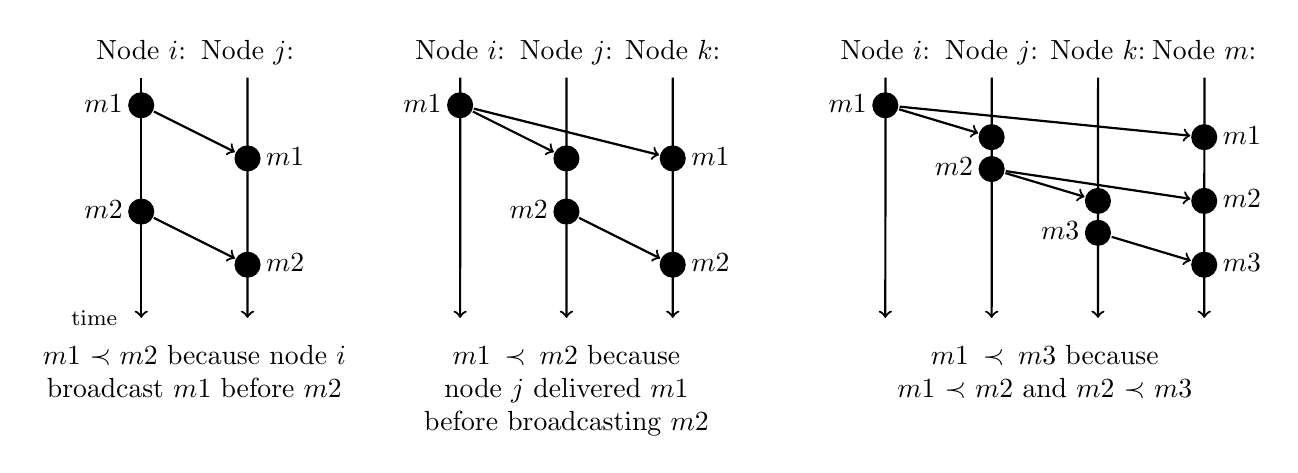
\begin{tikzpicture}[auto,scale=1.35]

\tikzstyle{event}=[circle,fill,minimum size=2pt]
\tikzstyle{label}=[text height=8pt,text depth=3pt]
\tikzstyle{leftlabel}=[label,left=3pt]
\tikzstyle{rightlabel}=[label,right=3pt]
\tikzstyle{every path}=[thick,->]
\tikzstyle{caption}=[text width=4cm,text centered,text height=8pt,below=5pt]

\node [label] (i1name) at (0,2.5) {Node $i$:};
\node [label] (j1name) at (1,2.5) {Node $j$:};
\node [event] (op1send) at (0,2.0) {};
\node [event] (op1recv) at (1,1.5) {};
\node [event] (op2send) at (0,1.0) {};
\node [event] (op2recv) at (1,0.5) {};
\node [leftlabel]  at (0,2.0) {$\isa{m1}$};
\node [rightlabel] at (1,1.5) {$\isa{m1}$};
\node [leftlabel]  at (0,1.0) {$\isa{m2}$};
\node [rightlabel] at (1,0.5) {$\isa{m2}$};
\draw (i1name) -- (0,0) node [left=5pt,at end] {\footnotesize time};
\draw (j1name) -- (1,0);
\draw (op1send) -- (op1recv);
\draw (op2send) -- (op2recv);
\node [caption] at (0.5,0) {
    $\isa{m1} \prec \isa{m2}$
    because node $i$ broadcast $\isa{m1}$ before $\isa{m2}$
};

\node [label] (i2name) at (3,2.5) {Node $i$:};
\node [label] (j2name) at (4,2.5) {Node $j$:};
\node [label] (k2name) at (5,2.5) {Node $k$:};
\node [event] (op3send) at (3,2.0) {};
\node [event] (op3recj) at (4,1.5) {};
\node [event] (op3reck) at (5,1.5) {};
\node [event] (op4send) at (4,1.0) {};
\node [event] (op4reck) at (5,0.5) {};
\node [leftlabel]  at (3,2.0) {$\isa{m1}$};
\node [rightlabel] at (5,1.5) {$\isa{m1}$};
\node [leftlabel]  at (4,1.0) {$\isa{m2}$};
\node [rightlabel] at (5,0.5) {$\isa{m2}$};
\draw (i2name) -- (3,0);
\draw (j2name) -- (4,0);
\draw (k2name) -- (5,0);
\draw (op3send) -- (op3recj);
\draw (op3send) -- (op3reck);
\draw (op4send) -- (op4reck);
\node [caption] at (4.0,0) {
    $\isa{m1} \prec \isa{m2}$
    because node $j$ delivered $\isa{m1}$ before broadcasting $\isa{m2}$
};

\node [label] (i3name) at  (7,2.5) {Node $i$:};
\node [label] (j3name) at  (8,2.5) {Node $j$:};
\node [label] (k3name) at  (9,2.5) {Node $k$:};
\node [label] (m3name) at (10,2.5) {Node $m$:};
\node [event] (op5send) at  (7,2.0) {};
\node [event] (op5recj) at  (8,1.7) {};
\node [event] (op5recm) at (10,1.7) {};
\node [event] (op6send) at  (8,1.4) {};
\node [event] (op6reck) at  (9,1.1) {};
\node [event] (op6recm) at (10,1.1) {};
\node [event] (op7send) at  (9,0.8) {};
\node [event] (op7recm) at (10,0.5) {};
\node [leftlabel]  at  (7,2.0) {$\isa{m1}$};
\node [rightlabel] at (10,1.7) {$\isa{m1}$};
\node [leftlabel]  at  (8,1.4) {$\isa{m2}$};
\node [rightlabel] at (10,1.1) {$\isa{m2}$};
\node [leftlabel]  at  (9,0.8) {$\isa{m3}$};
\node [rightlabel] at (10,0.5) {$\isa{m3}$};
\draw (i3name) -- (7,0);
\draw (j3name) -- (8,0);
\draw (k3name) -- (9,0);
\draw (m3name) -- (10,0);
\draw (op5send) -- (op5recj);
\draw (op5send) -- (op5recm);
\draw (op6send) -- (op6reck);
\draw (op6send) -- (op6recm);
\draw (op7send) -- (op7recm);
\node [caption] at (8.5,0) {
    $\isa{m1} \prec \isa{m3}$ because
    $\isa{m1} \prec \isa{m2}$ and
    $\isa{m2} \prec \isa{m3}$
};

\end{tikzpicture}
